% LTeX: language=es-es
\chapter{Trabajo realizado}
El trabajo realizado consistió en implementar y evaluar de forma empírica la estructura comprimida
simplificada para indexar texto basada en gramáticas simple propuesta en el libro \textit{Compact Data
Structures,(Indexed Searching in Grammar-Compressed Text)} \cite[Capítulo~10.5.6]{Navarro}. La implementación se encuentra disponible en el repositorio \textit{SimpleTextIndexingBasedOnGrammar}
\cite{SimpleTextIndexing}.

\section{Descripción General de la estructura}
La idea principal de la estructura es representar un diccionario $\mathcal{R}$ de \textit{r} reglas \textit{A} $\rightarrow$ \textit{BC} correspondiente a la gramática generada sobre un texto \textit{T} usando el algoritmo \textit{Re-Pair} como una grilla \textit{G} y una secuencia \textit{R} de símbolos que permite encontrar ocurrencias de patrones de texto en el texto original. 

La secuencia \textit{R} corresponde a la sucesión de reglas generadas por \textit{Re-Pair} expresadas como sus lados derechos, además de las reglas añadidas por la estructura con el fin de eliminar la secuencia \textit{C} generada por \textit{Re-Pair}.

La grilla en tanto corresponde a una grilla de $r \times r$ dimensiones con \textit{r} puntos que corresponden a las \textit{r} reglas predispuestos en la grilla de uan forma particular (explicada en las siguientes secciones) que permite obtener rangos de reglas que contienen ciertos patrones.

La búsqueda de patrones corresponde a primero encontrar en la grilla el área de esta que contiene los puntos correspondientes a reglas que expresan al patrón, que corresponde a la búsqueda primaria, para entonces obtener las posiciones de las ocurrencias como los desfases de cada uno de estos puntos con respecto respecto al símbolo inicial de la gramática extendida, llamada búsqueda secundaria de ocurrencias.

Las partes particulares y el detalle del proceso de búsqueda se explican en el presente texto, en las siguientes secciones.

\section{Diseño de la implementación}
Se implementó una clase \textit{facade} llamada \textit{\textbf{PatternSearcher}} que procesa la entrada e instancia las clases \textit{\textbf{ARSSequence}} (secuencia representada por permutaciones) y \textbf{\textit{Grid}} (grilla representada por matrices \textit{wavelet}), además de los otros miembros necesarios (como primitivas, vectores de bit, \textit{etc}.). \textit{PatternSearcher} expone, además de su constructor, un único método \textit{\textbf{search}} que corresponde a la búsqueda de patrones. 

El diagrama UML \ref{fig:uml} muestra el diseño general de la implementación.

\begin{figure}[h!]
    \centering
    \captionsetup{position=above} % Places the caption above the image
    \caption{Diagrama UML de la implementación}
    \includegraphics[width=1\textwidth]{imagenes/UML.png} % Adjust width as needed
    \label{fig:uml}
\end{figure}



\section{\textit{Re-Pair}}

La implementación de \textit{Re-Pair} de Shirou Maruyama\cite{re-pair} que utiliza las estrcuturas propuestas en la publicación original de Larsson \& Moffat\cite{Larsson2000}. Esta versión retorna una estructura que contiene un arreglo de reglas, además de la secuencia \textit{C} que corresponde a aquella que se obtiene una vez se aplican todas los reemplazos de las reglas en el texto original \textit{T}, y otros valores como la cantidad de reglas y el largo del texto (Véase \ref{lst:re-pair-call}). Las reglas corresponden a pares de enteros sin signo, donde los valores son menores a 256 si corresponden a una terminal o mayores si corresponden a una no terminal. Acceder a la posición 256 + $i$ del arreglo entrega la regla $i$.

\subsection{Generar reglas extras}
\label{sect:extrar}
Con objetivo de eliminar la secuencia \textit{C} para derivar el texto \textit{T} exclusivamente a partir de las reglas se crearon nuevas reglas $N_1 \rightarrow C[1] C[2]$, $N_2 \rightarrow C[3] C[4]$, $N_3 \rightarrow C[5] C[6]$, \textit{etc}, reemplazándolas en \textit{C}: $ N_1 N_2 N_3 ... N_{\lceil | C | /2 \rceil}$. Luego se hizo lo mismo con este nuevo \textit{C}, creando nuevas reglas $N^{'}_1 \rightarrow N_1 N_2$, $N^{'}_2 \rightarrow N_3 N_4$ y así sucesiva y recursivamente hasta obtener una única no terminal $S$ de la cual se puede derivar el texto original (Véase \ref{lst:rule-add}).

Sea $r = |\mathcal{R}|$ el número de reglas, y sea $A_i \rightarrow B_i C_i\; \forall\ 0\leq i < r$, el conjunto $\mathcal{R}$ es representado por la secuencia de enteros $R =  B_0 C_0 B_1 C_1 ... B_{r-1}C_{r-1}$. Nótese que la secuencia es auto-referencial: sea $R_i \rightarrow B_i C_i$, esta regla aparece en la secuencia en las posiciones $2i$ y $2i+1$, y reglas que deriven en $R_i$ tendrán uno de sus dos símbolos $B$ o $C$ con un valor 256 + $i$. 

Tómese en cuenta que en el trabajo presente cuando se habla de los lados izquierdo y derecho de una regla $R_i$, estos se refieren, respectivamente, a $B_i$ y $C_i$. También, cuando se hable de la compresión del texto a gramática, se hace referencia a la combinación de los procesos de comprimir por \textit{Re-Pair} seguido de la expansión de reglas con el fin de eliminar \textit{C}. 

La representación de la secuencia $R$, según las instrucciones del libro, utiliza permutaciones, y el detalle se explica más adelante, pero para hacer esta representación es necesario primero normalizar la secuencia de forma que los elementos en esta partan de 0 y sean continuos, es decir, el alfabeto de la secuencia no tiene saltos, y el mayor elemento es igual a la suma de las cantidades de terminales y no terminales menos 1.

\section{Normalizar secuencia}

Se creó un vector de bits \textit{b} (utilizando la librería \textit{SDSL}\cite{sdsl-lite}) de tamaño 256. La idea fue marcar con 1 las posiciones correspondientes a los símbolos terminales que aparecen en el texto \textit{T}, que son los símbolos terminales que aparecen en $R$. Esto conllevó a la restricción de que el texto debe tener formato donde cada carácter utiliza solo 1 byte (por ejemplo, UTF-8). Añadiendo suporte para \textit{Select}$_1$(\textit{i}) (reportar la posición del \textit{i}-ésimo uno en el vector) y \textit{Rank}$_1$(\textit{i}) (reportar la cantidad de unos hasta la posición \textit{i}) sobre el vector se puede obtener el símbolo original de la secuencia normalizada. Se guardan entonces los resultados de \textit{select} y \textit{rank} sobre el vector de bits, y estos dos vectores de largo 256 con elementos de tamaño 8 bits son los que se usarán en la estructura.

La secuencia normalizada ahora tiene símbolos entre 0 y la suma de las cantidades de terminales y no terminales menos 1. Elementos en la secuencia menores a la cantidad de terminales corresponden a símbolos terminales, mientras los demás corresponden a no terminales. La regla $R_i$ aparece en las posiciones $i$ y $i+1$ correspondiente a $B_i$ y $C_i$ respectivamente. Reglas que expanden a $R_i$ son las reglas $R_j$ donde alguno de sus $B_j$ o $C_j$ tienen como valor $i + $ número de terminales. El número de terminales es equivalente a \textit{rank}$_1$($b, |R|$). (Véase \ref{lst:normalizar})

Nótese que normalizar la secuencia es necesario solo para la implementación específica de \textit{Re-Pair} utilizada. En contraste, la versión de \textit{Re-Pair} de Navarro\cite{re-pair-navarro} normaliza automáticamente las reglas, entregando la secuencia \textit{C}, la secuencia \textit{R} de reglas, un valor numérico que indica la cantidad de símbolos terminales en el alfabeto usado en el texto y una secuencia numérica para obtener el símbolo original en el texto a partir del símbolo en la secuencia normalizada, exactamente como la implementación del trabajo presente.

\section{Secuencia utilizando permutaciones}

Se implementó la estructura descrita en el libro \cite[Capítulo~6.1]{Navarro} para representar secuencias de números utilizando permutaciones. Esta estructura permite las operaciones \textit{Access} y \textit{Rank} en tiempo $\mathcal{O}$(log log $\sigma$), donde $\sigma$ es el tamaño del alfabeto que compone la secuencia, y la operación \textit{Select} en tiempo $\mathcal{O}$(1). Esta última es importante pues es utilizada de forma frecuente en la búsqueda de ocurrencias secundarias en las reglas, lo cual será explicado más adelante.

\subsection{Permutaciones}

Una permutación $\pi$ de [1,n] es un reordenamiento de valores entre 1 y n. Descrita en el capítulo 5.1 \cite{Navarro}, la estructura que compete al trabajo realizado permite la operación $\pi^{-1}(i)$, esto es, la permutación inversa de $i$: encontrar un $j$ tal que $\pi(j) = i$ en tiempo $\mathcal{O}$(\textit{t}), donde \textit{t} es un parámetro de la estructura.

La idea de la estructura es aprovechar el concepto de descomposición en ciclos de la permutación. Si se aplica una permutación sobre un valor inicial se obtiene un segundo valor, y luego se aplica sobre este valor la permutación, y así sucesivamente, se terminará llegando al valor inicial. Este recorrido de valores se llama ciclo, y una permutación puede tener uno o más ciclos. 

Para calcular la permutación inversa de $i$ se aplica la permutación recursivamente hasta tener un $j$ cuya permutación es $i$. Esto requiere recorrer todo el ciclo que contiene a $i$. Sin embargo, si se guardan atajos de tamaño \textit{t}, con la idea de que si el elemento sobre el cual se está aplicando la permutación durante el recorrido del ciclo tiene un atajo, se toma ese atajo, saltándose una gran parte de los pasos recursivos, asegurando encontrar el inverso en no más de $t$ pasos.

Esta estructura se implemento satisfactoriamente utilizando los vectores de bit de la librería SDSL\cite{sdsl-lite} (Véase encabezado \ref{lst:perm}).

\subsection{Secuencia}

Dada la secuencia \textit{S} de tamaño \textit{n} sobre un alfabeto $\Sigma$, se divide esta, conceptualmente, en $\lceil n /\sigma \rceil$ pedazos $S_i = S[i \dots i+\sigma)$. Para resolver \textit{access}, \textit{rank} y \textit{select} se utilizan $\sigma$ vectores de bit $A_c$, con $c \in \Sigma$, donde $A_c = 1^{ rank_{c}(S_0, \sigma) } 0 1^{rank_{c}(S_1, \sigma)} \dots 0 1^{rank_{c}(S_{\lceil n /\sigma \rceil - 1}, \sigma)} $. En esencia, $A_c$ indica de forma unaria las ocurrencias del símbolo $c$ en casa pedazo de $S$. Con esto, las operaciones a nivel de los pedazos son:

Para todas $k = \lfloor i / \sigma \rfloor $.

\[ 
access(S, i) = access(S_k, i \ \text{mod} \ \sigma) 
\]
Para \textit{rank}, se debe calcular la cantidad de unos que aparecen en los pedazos anteriores al que corresponde a \textit{i}:
\[ 
rank_{c}(S, i) = 
\begin{cases} 
rank_{c}(S_k, i \ \text{mod} \ \sigma) & \text{si } k = 0,\\
rank_{c}(S_k, i \ \text{mod} \ \sigma) + select_{0}(A_{c}, k) - k & \text{si } k > 0
\end{cases} \]
Para \textit{select} se debe encontrar el pedazo al que pertenece el \textit{i} buscado, luego la respuesta es la suma de la posición donde parte este pedazo y \textit{select} sobre el pedazo, menos la posición del último cero antes del pedazo.
\[
select_{c}(S, j) = 
(s-j+1) \cdot \sigma +
select_{c}(S_{s-j+1}, s - \text{pred}_{0}(A_{c}, s)) \text{ donde } s = select_{1}(A_{c},j)
\]

Las operaciones dentro de cada pedazo \textit{C} requieren representar estos como la permutación inducida por su índice invertido. Sea $L_c$ la secuencia de las posiciones de los símbolos $c$ en el pedazo \textit{C}. Considérese la permutación $\pi = L_0 L_1 L_2 L_3 ... L_{\sigma-1}$ y las lista \textit{D} que marca las posiciones donde empieza cada lista en $\pi$, $D = 0^{|L_{0}|}10^{|L_{1}|} \dots 0^{|L_{\sigma-1}|}$

Utilizando la estructura anteriormente implementada se pueden resolver las operaciones dentro de los pedazos. Por ejemplo:

\[
access(C, i) = select_{0}(D, j) - j \text{, donde } j = \pi ^{-1}(i)
\]

Esta estructura se implementó correctamente (Véase el encabezado \ref{lst:seq})

\section{Reordenar secuencia}
\label{sec:reordenar}

La secuencia $R$ obtenida a partir de las reglas una vez completado el proceso de normalización es tal que estas reglas aparecen en el orden en que fueron creadas por el algoritmo \textit{Re-Pair} y extendidas con el fin de eliminar la secuencia \textit{C}. Lo que se quiere es que las reglas $R_i \rightarrow B_i C_i$ aparezcan ordenadas de forma creciente según el valor lexicográfico de la expansión inversa del lado izquierdo ($B_i$). 


La función de la librería estándar de C++ \textit{sort} puede ordenar la secuencia mientras se le otorgue una forma de expandir las reglas, pero esto no es suficiente pues se necesita que la secuencia de reglas mantenga la propiedad de auto-referencia, es decir, que cada regla $R_i$ aparezca en las posiciones $2i$ y $2i+1$ y que referencias a esta regla tenga el valor $i + \sigma$. Para lograr esto, se creó un vector de enteros que guarda los índices de cada regla. 

\begin{lstlisting}[style=cppstyle, caption={Vector de índices}, label={lst:example}]
int_vector reverseIndexMap(n_non_terminals);
for (int i = 0; i < n_non_terminals; i++) {
   reverseIndexMap[i] = i;
}
\end{lstlisting}

Luego se ordenó utilizando una función que compara las expansiones de los lados izquierdo de la regla apuntada por el índice, de forma inversa.
\begin{lstlisting}[style=cppstyle, caption={\textit{sort}}, label={lst:sort1}] 
sort(
    reverseIndexMap.begin(), 
    reverseIndexMap.end(), 
    [&](int a, int b) { 
        return compareRulesLazy(arsSequence, a, b, n_terminals, select, true); 
    }
);
\end{lstlisting}
La función de comparación es una función perezosa que entrega el siguiente símbolo de la expansión pedida a demanda, esto evita tener que expandir el lado requerido por completo, lo cual, en un texto largo con miles de reglas, puede llevar demasiado tiempo. Para esto se utilizaron generadores:

\begin{lstlisting}[style=cppstyle, caption={Comparación perezosa}, label={lst:cmp}] 
Generator<char> expandRuleSideLazy(
    ARSSequence& arrs, int i, int nt,
    std::vector<char>& sl, bool left = false)
{    
    int lr_i = left? i: i+1;
    if (arrs[lr_i] < nt) {
        co_yield sl[arrs[lr_i] + 1];
    } else {
        auto gen = expandRuleLazy(arrs, 2*(arrs[lr_i]-nt), nt, sl, left);
        for (char c : gen) {
            co_yield c;
        }
    }
}
bool compareRulesLazy(ARSSequence& arrs, int i, int j, int nt, std::vector<char>& sl, bool rev = false) 
{
    auto gen_i = expandRuleSideLazy(arrs, 2 * i, nt, sl, rev);
    auto gen_j = expandRuleSideLazy(arrs, 2 * j, nt, sl, rev);
    auto it_i = gen_i.begin();
    auto it_j = gen_j.begin();
    while (it_i != gen_i.end() && it_j != gen_j.end()) {
        char char_i = *it_i;
        char char_j = *it_j;
        if (char_i != char_j) {
            return char_i < char_j;
        }
        ++it_i;
        ++it_j;
    }
    // If one sequence is shorter, the shorter one is considered "less"
    return (it_i == gen_i.end()) && (it_j != gen_j.end());
}
\end{lstlisting}

Con esto, el vector \textit{reverseIndexMap} (rim) ahora contiene los índices de las reglas de forma tal que:
\[\forall i,j\ expansion\text{-}reversa (B_{rim[i]}) < expansion\text{-}reversa (B_{rim[i]})  \longleftrightarrow i < j \]
Se creó un vector del mismo tamaño que $R$ y se colocaron en este las reglas en el orden que aparecen en \textit{reverseIndexMap}, pero actualizando los valores $B$ y $C$:
\begin{lstlisting}[style=cppstyle, caption={\textit{Nueva secuencia R}}, label={lst:sort2}] 
vector<int> distance_of_find(reverseIndexMap.size(), 0);
for (int i = 0; i < reverseIndexMap.size(); i++) {
    distance_of_find[reverseIndexMap[i]] = i;        
}
int_vector<> sortedSequenceR = int_vector(n_non_terminals * 2 + 1, 0);
for (u_int i = 0; i < reverseIndexMap.size(); i++) {        
    int a_i = reverseIndexMap[i]; 
    int b_i = normalized_sequenceR[a_i*2];
    int c_i = normalized_sequenceR[a_i*2+1];
    int n_b_i, n_c_i;
    if (b_i < n_terminals) {
        n_b_i = b_i;
    } else {
        n_b_i = distance_of_find[b_i - n_terminals]  + n_terminals;
    }
    if (c_i < n_terminals) {
        n_c_i = c_i;
    } else {
        n_c_i = distance_of_find[c_i - n_terminals] + n_terminals;
    }
    sortedSequenceR[i*2] = n_b_i; 
    sortedSequenceR[i*2+1] = n_c_i; 
} 
int S_i = distance(reverseIndexMap.begin(), find(reverseIndexMap.begin(), reverseIndexMap.end(), n_non_terminals-1));  
sortedSequenceR[n_non_terminals*2] = S_i; 
R = ARSSequence(sortedSequenceR, max_normalized + 1 + 1);
\end{lstlisting}
La última linea guarda el índice de la regla inicial (anteriormente, la regla inicial era aquella expresada por los dos últimos valores en \textit{R}, ahora debe guardarse su posición).

Se creó también un vector similar a \textit{reverseIndexMap}, llamado \textit{indexMap} que guarda los índices de las reglas en el arreglo anteriormente ordenado, ordenadas por el valor lexicográfico de la expansión (no inversa) del lado derecho de cada regla. Este vector se utilizará para crear la grilla.

\subsection{Memoización}

Es posible aplicar la técnica de memoización para reducir el tiempo de la función de comparación, al guardar los valores de las expansiones de las reglas:

\begin{lstlisting}[style=cppstyle, caption={\textit{Nueva secuencia R}}, label={lst:sort3}] 
vector<int> distance_of_find(reverseIndexMap.size(), 0);
for (int i = 0; i < reverseIndexMap.size(); i++) {
    distance_of_find[reverseIndexMap[i]] = i;        
}
int_vector<> sortedSequenceR = int_vector(n_non_terminals * 2 + 1, 0);
for (u_int i = 0; i < reverseIndexMap.size(); i++) {        
    int a_i = reverseIndexMap[i]; 
    int b_i = normalized_sequenceR[a_i*2];
    int c_i = normalized_sequenceR[a_i*2+1];
    int n_b_i, n_c_i;
    if (b_i < n_terminals) {
        n_b_i = b_i;
    } else {
        n_b_i = distance_of_find[b_i - n_terminals]  + n_terminals;
    }
    if (c_i < n_terminals) {
        n_c_i = c_i;
    } else {
        n_c_i = distance_of_find[c_i - n_terminals] + n_terminals;
    }
    sortedSequenceR[i*2] = n_b_i; 
    sortedSequenceR[i*2+1] = n_c_i; 
} 
int S_i = distance(reverseIndexMap.begin(), find(reverseIndexMap.begin(), reverseIndexMap.end(), n_non_terminals-1));  
sortedSequenceR[n_non_terminals*2] = S_i; 
R = ARSSequence(sortedSequenceR, max_normalized + 1 + 1);
\end{lstlisting}

Esto sin embargo requiere mucho espacio extra y no comprime el texto, por lo que no es parte de la estructura, sin embargo posibles casos de utilidad son discutidos al final del trabajo.

\section{Ejemplo práctico}

Considérese el texto $T =$ \textit{abrabracadabrabra} y su versión normalizada:
\[T = 0\ 1\ 4\ 0\ 1\ 4\ 0\ 2\ 0\ 3\ 0\ 1\ 4\ 0\ 1\ 4\ 0
\]
Considérese también la gramática representada por la secuencia \textit{R}, normalizada y reordenada:
\[ R = 0\ 9\ 8\ 11\ 5\ 9\ 7\ 10\ 1\ 12\ 2\ 0\ 3\ 7\ 4\ 0  \] 
Donde la regla inicial es $R_1 = 8\ 11$.

Sea $s(i) = select_{1}(b, i + 1)$ ($b$ es el vector de bits obtenido durante la normalización de la secuencia) y $\sigma$ el tamaño del alfabeto de terminales (en este caso, con $\Sigma = $ [0, 1, 2, 3, 4] se tiene $\sigma = 5$), la figura \ref{fig:transformaciones} ilustra la expansión de las reglas, con $R_1$ la regla inicial que expande al texto original.
\begin{figure}[ht]
\centering

$R = 0\ 9\ 8\ 11\ 5\ 9\ 7\ 10\ 1\ 12\ 2\ 0\ 3\ 7\ 4\ 0$ \\
$(R = a R_4\ R_3 R_6\ R_0 R_4\ R_2 R_5\ b R_7\ c a\ d R_2\ r a)$
\[
\begin{array}{rl}
R_0 & \rightarrow 0\ 9 
\Longleftrightarrow s(0)\ R_{9 - \sigma} \Longleftrightarrow \textbf{a}\ R_{4} \Longleftrightarrow  \textbf{a} \text{ bra} \\
R_1 & \rightarrow 8\ 11\ 
\Longleftrightarrow R_{8 - \sigma}\ R_{11 - \sigma} \Longleftrightarrow R_{3}\ R_{6} \Longleftrightarrow \textbf{abrabraca} \text{ dabrabra} \\
R_2 & \rightarrow 5\ 9\ 
\Longleftrightarrow R_{5 - \sigma}\ R_{9 - \sigma} \Longleftrightarrow R_{0}\ R_{4} \Longleftrightarrow \textbf{abra} \text{ bra} \\
R_3 & \rightarrow 7\ 10\ 
\Longleftrightarrow R_{7 - \sigma}\ R_{10 - \sigma} \Longleftrightarrow R_{2}\ R_{5} \Longleftrightarrow \textbf{abrabra} \text{ ca} \\
R_4 & \rightarrow 1\ 12\ 
\Longleftrightarrow s(1)\ R_{12 - \sigma} \Longleftrightarrow \textbf{b}\ R_{7} \Longleftrightarrow \textbf{b} \text{ ra} \\
R_5 & \rightarrow 2\ 0\ 
\Longleftrightarrow s(2)\ s(0) \Longleftrightarrow \textbf{c} \text{ a} \\
R_6 & \rightarrow 3\ 7\ 
\Longleftrightarrow s(3)\ R_{7 - \sigma} \Longleftrightarrow \textbf{d}\ R_2 \Longleftrightarrow \textbf{d} \text{ abrabra} \\
R_7 & \rightarrow 4\ 0 
\Longleftrightarrow s(4)\ s(0) \Longleftrightarrow \textbf{r} \text{ a} \\
\end{array}
\]
$l = 4\ 17\ 7\ 9\ 3\ 2\ 8\ 2$
\caption{Secuencia \textit{R} y expansión de las reglas $R_i$, junto con secuencia \textit{l}, el largo de cada expansión}
\label{fig:transformaciones}
\end{figure}

Como se aprecia al expandir cada regla, estas están ordenadas de forma ascendente por el valor lexicográfico de la expansión invertida del lado izquierdo (en negrita).

Es posible visualizar esta gramática como un \textbf{árbol sintáctico} o \textit{parsing tree} (Véase figura \ref{fig:tree}) que se obtiene de recorrer \textit{R} desde la regla inicial $R_1$. Esta figura permite visualizar la idea de \textbf{Gramática Balanceada}: en una gramática balanceada, la altura del árbol sintáctico es del orden $\mathcal{O}(\log n)$, con \textit{n} es el largo del texto original, es decir, existe una constante \textit{c} tal que la altura es $\leq c \log n$ para todos los textos de largo \textit{n}. 

Para que la gramática representada por \textit{R} sea balanceada es menester que la implementación de \textit{Re-Pair} genere una gramática balanceada, luego la expansión de las reglas es balanceada naturalmente.

\begin{figure}[ht]
\centering
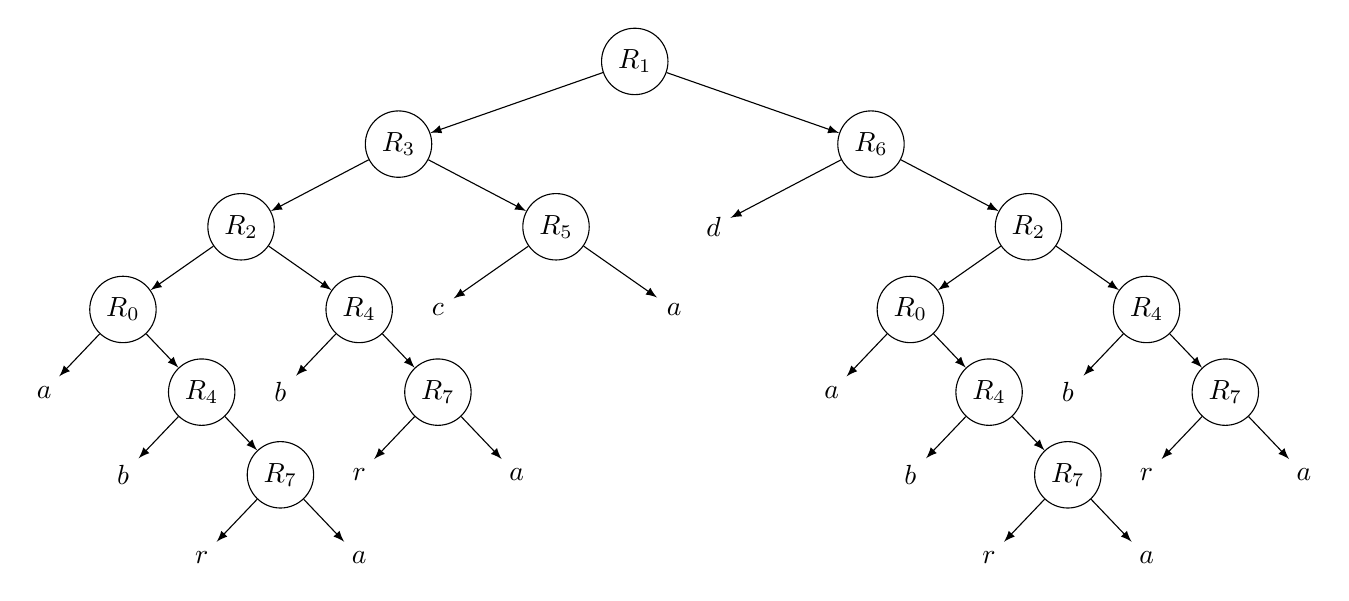
\begin{tikzpicture}[
    level distance=1.05cm, % Increases the vertical spacing
    level 1/.style={sibling distance=6cm}, % Adjust sibling spacing for top level
    level 2/.style={sibling distance=4cm},
    level 3/.style={sibling distance=3cm},
    level 4/.style={sibling distance=2cm},
    level 5/.style={sibling distance=2cm}, % Add specific spacing for deeper levels
    edge from parent/.style={draw, -latex}
]

% Root node
\node (R1) [circle, draw]{\( R_1 \)}
    child {node[circle, draw] {\( R_{3} \)}
        child {node[circle, draw] {\( R_2 \) }
            child {node[circle, draw]{\( R_0 \)}
                child {node{\( a \)}}
                    child {node[circle, draw]{\( R_4 \)}
                        child {node{\( b \)}}
                        child {node[circle, draw]{\( R_7 \)}
                            child {node{\( r \)}}
                            child {node{\( a \)}}
                        }
                    }
            }
            child {node[circle, draw]{\( R_4 \)}
                child {node{\( b \)}}
                child {node[circle, draw]{\( R_7 \)}
                    child {node{\( r \)}}
                    child {node{\( a \)}}
                }
            }
        }
        child {node[circle, draw] {\( R_5 \)}
            child {node {\( c \)  }}
            child {node {\( a \)  }}
        }
    }
    child {node[circle, draw] {\( R_6 \)}
        child {node {\( d \)   }}
        child {node[circle, draw] {\( R_2 \)  }
            child {node[circle, draw]{\( R_0 \)}
                child {node{\( a \)}}
                child {node[circle, draw]{\( R_4 \)}
                    child {node{\( b \)}}
                    child {node[circle, draw]{\( R_7 \)}
                        child {node{\( r \)}}
                        child {node{\( a \)}}
                    }
                }
            }
            child {node[circle, draw]{\( R_4 \)}
                child {node{\( b \)}}
                child {node[circle, draw]{\( R_7 \)}
                    child {node{\( r \)}}
                    child {node{\( a \)}}
                }
            }
        }
    };

\end{tikzpicture}
\caption{Árbol sintáctico para \textit{abrabracadabrabra}}
\label{fig:tree}
\end{figure}

Otra visualización de la gramática que será de utilidad para visualizar la búsqueda de patrones es la de un grafo acíclico dirigido o DAG (del inglés \textit{Directed Acyclic Graph}) (Fígura \ref{fig:DAG}). 

El DAG se forma de la siguiente forma. Cada regla tiene un único nodo correspondiente en el grafo. Cada vez que una regla $R_i$ aparece ya sea como lado izquierdo o derecho de otra regla $R_j$, esto induce una conexión desde el nodo $R_i$ al nodo $R_j$. El único nodo sin conexiones salientes corresponde a la regla inicial, en este caso, $R_1$.

\begin{figure}[H]
\begin{tikzpicture}[
	roundnode/.style={circle, draw=gray!100, thick, minimum size=6mm},
    squarenode/.style={rectangle, draw=gray!100, thick, minimum size=6mm},]
	
	\node[roundnode,font=\bfseries\sffamily] (R1) at (5.5,0) {$R_1$};
    
	\node[roundnode,font=\bfseries\sffamily] (R3) at (4,-0.9) {$R_3$};
	\node[roundnode,font=\bfseries\sffamily] (R6) at (7,-1) {$R_6$};
    
	\node[roundnode,font=\bfseries\sffamily] (R2) at (3,-2.3) {$R_2$};
    \node[roundnode,font=\bfseries\sffamily] (R5) at (5,-2.3) {$R_5$};
    \node[squarenode,font=\bfseries\sffamily] (d) at (6,-2.3) {$d$};

    \node[roundnode,font=\bfseries\sffamily] (R0) at (2,-3.5) {$R_0$};
    \node[roundnode,font=\bfseries\sffamily] (R4) at (3.4,-4.4) {$R_4$};
    \node[squarenode,font=\bfseries\sffamily] (c) at (4.1,-3.5) {$c$};

    \node[roundnode,font=\bfseries\sffamily] (R7) at (4.4,-5.8) {$R_7$};
    \node[squarenode,font=\bfseries\sffamily] (b) at (3.0,-5.8) {$b$};

    \node[squarenode,font=\bfseries\sffamily] (r) at (3.9,-7.0) {$r$};
    \node[squarenode,font=\bfseries\sffamily] (a) at (5.2,-7.0) {$a$};
	
	\draw [->, gray, -{Latex[length=1.5mm, width=2mm]}] (R3) to (R1);
    \draw [->, black, -{Latex[length=1.5mm, width=2mm]}] (R6) to (R1);
    
    \draw [->, gray, -{Latex[length=2mm, width=2mm]}] (R2) to (R3);
    \draw [->, black, -{Latex[length=1.5mm, width=2mm]}] (R5) to (R3);
    \draw [->, gray, -{Latex[length=2mm, width=2mm]}] (d) to (R6);  
    \draw [->, black, -{Latex[length=2mm, width=2mm]}] (R2) to[out=45, in=315] (R6);

    \draw [->, gray, -{Latex[length=2mm, width=2mm]}] (R0) to (R2);
    \draw [->, black, -{Latex[length=2mm, width=2mm]}] (R4) to[out=90, in=315] (R2);
    \draw [->, black, -{Latex[length=2mm, width=2mm]}] (R4) to (R0);
    \draw [->, gray, -{Latex[length=2mm, width=2mm]}] (c) to (R5);

    \draw [->, gray, -{Latex[length=2mm, width=2mm]}] (a) to[out=225, in=225] (R0);
    \draw [->, black, -{Latex[length=2mm, width=2mm]}] (a) to[out=30, in=315] (R5);
    \draw [->, black, -{Latex[length=2mm, width=2mm]}] (a) to (R7);
    \draw [->, gray, -{Latex[length=2mm, width=2mm]}] (r) to (R7);

    \draw [->, gray, -{Latex[length=2mm, width=2mm]}] (b) to (R4);
    \draw [->, black, -{Latex[length=2mm, width=2mm]}] (R7) to (R4);
	
	
\end{tikzpicture}
\caption{DAG para \textit{abrabracadabrabra}, las conexiones que corresponden a reglas que aparecen como lados izquierdos son grises, y las derechas son negras}
\label{fig:DAG}
\end{figure}


\newpage
\section{Grilla}

\textit{Compact Data Structures}\cite{Navarro} describe en su décimo capítulo la estructura de grilla en base a árboles \textit{wavelet} (más precisamente, las estructuras utilizan matrices \textit{wavelet}, pero los algoritmos descritos en el libro utilizan árboles). Para esto primero se ordenan los puntos de entrada por la coordenada \textit{x}. Luego, cada punto $(x_i, y_i)$ es representado en la grilla por el punto $(i, y_i)$. El mapeo entre los puntos originales y los nuevos se guarda en un vector de bits, sin embargo, esto es innecesario para el caso presente debido a que los valores $x_i$ son únicos y continuos, con lo cual al ordenar los puntos por \textit{x}, $(x_i, y_i) = (i, y_i)$. Una vez se tienen los puntos ordenados, si se consideran ahora solo los valores $y_i$ de cada punto, se tiene una secuencia \textit{S}. Es a partir de esta secuencia que se crea la matriz \textit{wavelet}\cite[Capítulo 6.2.5]{Navarro}.

\subsection{Matrices \textit{Wavelet}}

La idea de la matriz \textit{wavelet} es concatenar todos los vectores de bits en un mismo nivel para deshacerse de la topología de árbol. La forma particular en que son concatenados los vectores busca evitar espacios vacíos que aparecen en el árbol (pues no todos los caminos raíz-hoja tienen el mismo largo) es la siguiente: se colocan primero los vectores de bits correspondientes a hijos izquierdos del nivel anterior y luego los hijos derechos. Por ejemplo, para la secuencia "\textit{tobeornottobethatisthequestion}":

\[
\begin{array}{lcll}
S_1 & : & \texttt{tobeornottobethatisthequestion} & \\
B_1 & : & \texttt{110011011110010010110011011010} & z_1 = 13 \\[10pt]
S_2 & : & \texttt{benbehaiheein toorottottstqusto} & \\
B_2 & : & \texttt{0010010110011 10000110111101110} & z_2 = 14 \\[10pt]
S_3 & : & \texttt{bebeaee oorooqo nhihin tttttstust } & \\
B_3 & : & \texttt{0101011 0010000 100001 0000000100 } & z_3 = 22 \\[10pt]
S_4 & : & \texttt{bba ooooqo hihi tttttstst eeee r nn u} & \\
B_4 & : & \texttt{110 000010 0101 111110101 } & z_4 = 10 \\[10pt]
S_5 & : & \texttt{a ooooo hh ss bb q ii ttttttt} & \\
\end{array}
\]

Donde $z_l$ es un valor pre-calculado equivalente a $Rank_0 (B_{l}, n)$.

La estructura y sus operaciones se implementaron correctamente (Véase \ref{lst:wlmt}) siguiendo las instrucciones del capítulo 6.2.5 de \textit{Compact Data Structures}\cite{Navarro}. Con esto, se implementó la estructura de grilla usando matrices \textit{wavelet}\cite[Capítulo 10.1]{Navarro} (Véase \ref{lst:grid}).

\subsection{Preparar puntos para grilla}

Cada regla $R_i \rightarrow B_i C_i $ se guarda en la grilla en un punto con coordenadas $(B_i, C_i)$. Las filas de la grilla están ordenadas por orden lexicográfico del reverso de la expansión de $B_i$ (esto ya se hizo). Las columnas en tanto están ordenadas por orden lexicográfico de la expansión de $C_i$. Para lograr esto se usó el vector \textit{indexMap} descrito previamente:
\begin{lstlisting}[style=cppstyle] 
std::vector<Point> points(n_non_terminals);
u_int j, k;
for (u_int i = 0; i < indexMap.size(); i++) {
    k = std::distance(indexMap.begin(), std::find(indexMap.begin(), indexMap.end(), i));
    points[i] = Point(k, i);
}    
\end{lstlisting}

Estos puntos se usaron para inicializar la grilla (La implementación de la grilla usa valores indexados desde 1, por lo que hay que sumar 1 a los valores de los puntos antes de usarlos).

Por ejemplo, las reglas generadas por "\textit{abrabracadabrabra}" (Véase la fígura \ref{fig:transformaciones}), conforman la siguiente grilla:

\begin{figure}[h]
    \centering
    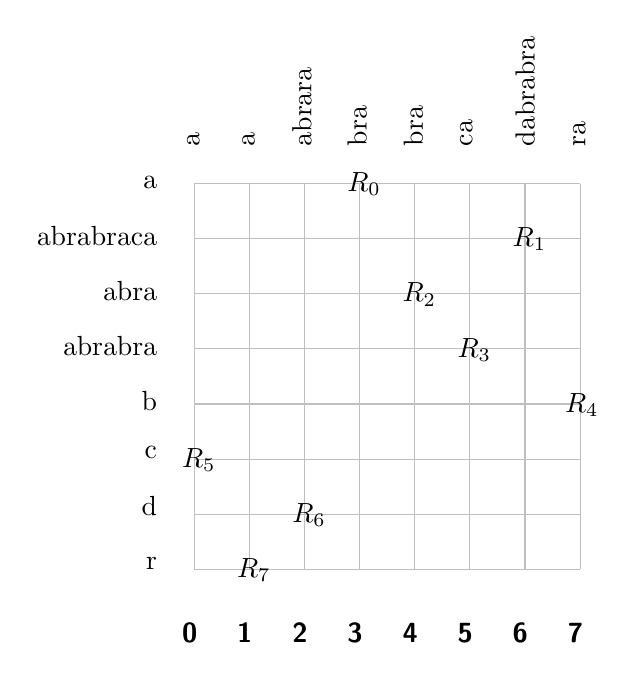
\begin{tikzpicture}[scale=0.7]% Draw the grid
	\draw[step=1cm,gray,opacity=0.5] (0,0) grid (7,7);	
	\node[anchor=north west,rotate=90] at (0-0.3, 7.5) {a};
	\node[anchor=north west,rotate=90] at (1-0.3, 7.5) {a};
	\node[anchor=north west,rotate=90] at (2-0.4, 7.5) {abrara};
	\node[anchor=north west,rotate=90] at (3-0.4, 7.5) {bra};
	\node[anchor=north west,rotate=90] at (4-0.38, 7.5) {bra};
	\node[anchor=north west,rotate=90] at (5-0.35, 7.5) {ca};
	\node[anchor=north west,rotate=90] at (6-0.35, 7.5) {dabrabra};
	\node[anchor=north west,rotate=90] at (7-0.3, 7.5) {ra};	
	\node[anchor=north east] at (-0.5,7+0.3) {a};
	\node[anchor=north east] at (-0.5,6+0.4) {abrabraca};
	\node[anchor=north east] at (-0.5,5+0.4) {abra};
	\node[anchor=north east] at (-0.5,4+0.4) {abrabra};
	\node[anchor=north east] at (-0.5,3+0.4) {b};
	\node[anchor=north east] at (-0.5,2+0.4) {c};
	\node[anchor=north east] at (-0.5,1+0.5) {d};
	\node[anchor=north east] at (-0.5,0+0.4) {r};
	%\pattern[pattern=north west lines, pattern color=gray] (0.0-0.2,4.0-0.3) rectangle (7.0+0.2,7.0+0.3);
	%\draw[red, thick] (0.0-0.2,4.0-0.3) rectangle (7.0+0.2,7.0+0.3);
	
	%\pattern[pattern=north east lines, pattern color=gray] (3.0-0.2,0.0-0.3) rectangle (4.0+0.3,7.0+0.4);
	%\draw[blue, thick] (3.0-0.3,0.0-0.3) rectangle (4.0+0.3,7.0+0.4);	
	\node[anchor=south west, text=black, font=\bfseries\sffamily] at (0.0-0.4,2.0-0.4) {$R_5$};
	\node[anchor=south west, text=black, font=\bfseries\sffamily] at (1.0-0.4,0.0-0.4) {$R_7$};
	\node[anchor=south west, text=black, font=\bfseries\sffamily] at (2.0-0.4,1.0-0.4) {$R_6$};
	\node[anchor=south west, text=black, font=\bfseries\sffamily] at (3.0-0.4,7.0-0.4) {$R_0$};
	\node[anchor=south west, text=black, font=\bfseries\sffamily] at (4.0-0.4,5.0-0.4) {$R_2$};
	\node[anchor=south west, text=black, font=\bfseries\sffamily] at (5.0-0.4,4.0-0.4) {$R_3$};
	\node[anchor=south west, text=black, font=\bfseries\sffamily] at (6.0-0.4,6.0-0.4) {$R_1$};
	\node[anchor=south west, text=black, font=\bfseries\sffamily] at (7.0-0.45,3.0-0.4) {$R_4$};
    
    \node[anchor=south west, text=black, font=\bfseries\sffamily] at (0-0.4,-1-0.5) {0};
    \node[anchor=south west, text=black, font=\bfseries\sffamily] at (1-0.4,-1-0.5) {1};
    \node[anchor=south west, text=black, font=\bfseries\sffamily] at (2-0.4,-1-0.5) {2};
    \node[anchor=south west, text=black, font=\bfseries\sffamily] at (3-0.4,-1-0.5) {3};
    \node[anchor=south west, text=black, font=\bfseries\sffamily] at (4-0.4,-1-0.5) {4};
    \node[anchor=south west, text=black, font=\bfseries\sffamily] at (5-0.4,-1-0.5) {5};
    \node[anchor=south west, text=black, font=\bfseries\sffamily] at (6-0.4,-1-0.5) {6};
    \node[anchor=south west, text=black, font=\bfseries\sffamily] at (7-0.4,-1-0.5) {7};
\end{tikzpicture}
    
    \caption{Grilla}
    \label{fig:grid}
\end{figure}


Si se lee la grilla fila por fila aparecen las reglas en este orden: $R_0, R_1, R_2, ... R_7$, es decir, en el orden preexistente, pues ya fueron ordenadas por orden lexicográfico de la expansión reversa del lado izquierdo (mostrado en la figura a la izquierda de cada fila). Si se leen las reglas columna a columna, el orden es $R_5, R_7, R_6, R_0, R_2, R_3, R_1, R_4$, pues las columnas están ordenadas por orden lexicográfico de la expansión del lado derecho (mostrado arriba de la grilla sobre cada columna correspondiente).

\section{Calcular largo de las expansiones de las reglas}

Es menester, para poder responder consultas de búsqueda de patrones, pre-calcular los valores de los largos de las expansiones de cada regla. El detalle se ve más adelante, pero en resumen, si una ocurrencia de un patrón sucede en una regla que aparece como el lado derecho $C_i$ de otra regla, el índice del patrón estará desfasado $l_{B_i}$ con respecto al índice de la regla padre, donde $l_{B_i}$ es el largo de la expansión de la regla $B_i$ que es el lado izquierdo de la regla $R_i$. 

\begin{lstlisting}[style=cppstyle]
l = int_vector(n_non_terminals, 0); // largos de cada regla
for (int i = 0; i < n_non_terminals; i++) {
    l[i] = ruleLength(i);
}
\end{lstlisting}

Como las reglas son referenciadas por otras reglas (y dependiendo de lo repetitivo del texto, son referenciadas más de una vez), con el fin de evitar calcular el largo para una misma regla cada vez que esta es parte de la expansión de otra, se usó \textit{memoización} (en este caso, la misma lista de largos funciona como la memoria).

\begin{lstlisting}[style=cppstyle]
int PatternSearcher::ruleLength(int_vector<> *l, int i) {
    if (l[i] != 0) { //memoization
        return l[i];
    }
    int left, right;
    if (R[i*2] < nt) {
        left = 1;
    } else {
        left = ruleLength(R[i*2] - nt);
    }
    if (R[i*2+1] < nt) {
        right = 1;
    } else {
        right = ruleLength(R[i*2+1] - nt);
    }
    l[i] = left + right;
    return l[i];
}
\end{lstlisting}

\section{Búsqueda de patrones}

La búsqueda de patrones aprovecha la grilla para encontrar las reglas en las que aparece el patrón de texto buscado. La idea es la siguiente: si el patrón $P$ a buscar aparece en el texto, entonces existe al menos una división del patrón $P$ en dos \textit{strings} $P_<$ y $P_>$ que son prefijo y sufijo del patrón respectivamente y que concatenados forman el patrón $P$, tales que $P_<$ es sufijo de la expansión izquierda de una regla $R_i$ y $P_>$ es prefijo de la expansión derecha de la misma regla. Si se tienen todas las reglas que cumplen esta condición, basta con recorrer virtualmente el árbol sintáctico o \textit{parsing tree} hasta el símbolo inicial, y entregar la posición donde parte $P_<$ tomando en cuenta los desfases con respecto al nodo padre. 

La idea entonces es, primero, y por cada división $P_<$ y $P_>$ del patrón, encontrar todas la reglas que expresan el patrón de la forma descrita (ocurrencias primarias), y luego, por cada una de estas reglas encontradas, hacer accesos en \textit{R} hasta encontrar todas las posiciones de esta regla en el símbolo inicial (ocurrencias secundarias). El detalle se ve en las siguientes secciones.

\subsection{Ocurrencias primarias}

Para cada posible división del patrón \textit{P} en dos \textit{strings}, uno prefijo y otro sufijo $P_<$ y $P_>$, se buscan las reglas cuya expansión izquierda es $P_<$ y derecha $P_>$.

Como las filas están ordenadas por orden lexicográfico de la expansión reversa del lado izquierdo de estas, las reglas que cuyo lado izquierdo terminan en $P_<$ forman un rango de filas en la grilla. De forma análoga, las columnas están ordenadas de forma lexicográfica por la expansión del lado derecho, por lo que las reglas con lado derecho que empieza con $P_>$ forman un rango de columnas. Esto significa que se puede encontrar el rango de filas y columnas (y por lo tanto, el cuadrante donde se encuentran las reglas que cumplen con la condición buscada) usando búsqueda binaria.

Por ejemplo, sea el patrón de búsqueda $P =$ \textbf{ab} sobre el texto \textit{abrabracadabrabra}, se tienen los posibles (y en este caso únicos) $P_< =$ \textbf{a} y $P_> =$ \textbf{b}. Las reglas que tienen como sufijo en su extensión izquierda a $P_< =$ \textbf{a} están en el rango de filas [$0,1,2,3$] (en ázul en la figura \ref{fig:grid-2}), mientras que las reglas que tienen como prefijo en el lado derecho a $P_> =$ \textbf{b} están en el rango de columnas [$3, 4$] (en rojo en la figura \ref{fig:grid-2}).

\begin{figure}[h]
    \centering
    \begin{tikzpicture}[scale=0.7]% Draw the grid
	\draw[step=1cm,gray,opacity=0.5] (0,0) grid (7,7);	
	\node[anchor=north west,rotate=90] at (0-0.3, 7.5) {a};
	\node[anchor=north west,rotate=90] at (1-0.3, 7.5) {a};
	\node[anchor=north west,rotate=90] at (2-0.4, 7.5) {abrara};
	\node[anchor=north west,rotate=90] at (3-0.4, 7.5) {bra};
	\node[anchor=north west,rotate=90] at (4-0.38, 7.5) {bra};
	\node[anchor=north west,rotate=90] at (5-0.35, 7.5) {ca};
	\node[anchor=north west,rotate=90] at (6-0.35, 7.5) {dabrabra};
	\node[anchor=north west,rotate=90] at (7-0.3, 7.5) {ra};	
	\node[anchor=north east] at (-0.5,7+0.3) {a};
	\node[anchor=north east] at (-0.5,6+0.4) {abrabraca};
	\node[anchor=north east] at (-0.5,5+0.4) {abra};
	\node[anchor=north east] at (-0.5,4+0.4) {abrabra};
	\node[anchor=north east] at (-0.5,3+0.4) {b};
	\node[anchor=north east] at (-0.5,2+0.4) {c};
	\node[anchor=north east] at (-0.5,1+0.5) {d};
	\node[anchor=north east] at (-0.5,0+0.4) {r};
	\pattern[pattern=north west lines, pattern color=blue, opacity=0.5] (0.0-0.2,4.0-0.3) rectangle (7.0+0.2,7.0+0.3);
	%\draw[red, thick] (0.0-0.2,4.0-0.3) rectangle (7.0+0.2,7.0+0.3);
	
	\pattern[pattern=north east lines, pattern color=red, opacity=0.5] (3.0-0.2,0.0-0.3) rectangle (4.0+0.3,7.0+0.4);
	%\draw[blue, thick] (3.0-0.3,0.0-0.3) rectangle (4.0+0.3,7.0+0.4);	
	\node[anchor=south west, text=black, font=\bfseries\sffamily] at (0.0-0.4,2.0-0.4) {$R_5$};
	\node[anchor=south west, text=black, font=\bfseries\sffamily] at (1.0-0.4,0.0-0.4) {$R_7$};
	\node[anchor=south west, text=black, font=\bfseries\sffamily] at (2.0-0.4,1.0-0.4) {$R_6$};
	\node[anchor=south west, text=black, font=\bfseries\sffamily] at (3.0-0.4,7.0-0.4) {$R_0$};
	\node[anchor=south west, text=black, font=\bfseries\sffamily] at (4.0-0.4,5.0-0.4) {$R_2$};
	\node[anchor=south west, text=black, font=\bfseries\sffamily] at (5.0-0.4,4.0-0.4) {$R_3$};
	\node[anchor=south west, text=black, font=\bfseries\sffamily] at (6.0-0.4,6.0-0.4) {$R_1$};
	\node[anchor=south west, text=black, font=\bfseries\sffamily] at (7.0-0.45,3.0-0.4) {$R_4$};
    
    \node[anchor=south west, text=black, font=\bfseries\sffamily] at (0-0.4,-1-0.5) {0};
    \node[anchor=south west, text=black, font=\bfseries\sffamily] at (1-0.4,-1-0.5) {1};
    \node[anchor=south west, text=black, font=\bfseries\sffamily] at (2-0.4,-1-0.5) {2};
    \node[anchor=south west, text=black, font=\bfseries\sffamily] at (3-0.4,-1-0.5) {3};
    \node[anchor=south west, text=black, font=\bfseries\sffamily] at (4-0.4,-1-0.5) {4};
    \node[anchor=south west, text=black, font=\bfseries\sffamily] at (5-0.4,-1-0.5) {5};
    \node[anchor=south west, text=black, font=\bfseries\sffamily] at (6-0.4,-1-0.5) {6};
    \node[anchor=south west, text=black, font=\bfseries\sffamily] at (7-0.4,-1-0.5) {7};
\end{tikzpicture}
    
    \caption{Grilla}
    \label{fig:grid-2}
\end{figure}

Las reglas $R_0$ y $R_2$ se encuentran en el cuadrante definido por los dos rangos encontrados. Estas reglas pueden obtenerse mediante la operación \textit{report} de la grilla. El siguiente paso es determinar los índices de las reglas en el texto original (Véase sección \ref{sect:second}). 

\subsubsection{Implementación}

La búsqueda de las reglas que contienen el patrón consiste en primero dividir este en dos \textit{sub-strings} ($P_<, P_>$), según una variable \textit{t} (el largo de $P_<$). Por cada \textit{t} entre 1 y el largo del patrón menos uno, se deben encontrar $s_y$ (primera fila del rango de filas), $e_y$ (última fila del rango), $s_x$ (primera columna del rango de columnas) y $e_x$ (última columna del rango).

\begin{lstlisting}[style=cppstyle]
u_int m = P.size();
u_int t;
for (t = 1; t < m; t++) {
    string P_left = P.substr(0, t); // P_<
    string P_right = P.substr(t, m-t); // P_>
    uint s_x, e_x, s_y, e_y;
\end{lstlisting}

Para buscar los rangos $s_x, e_x, s_y, e_y$ , se utilizó búsqueda binaria, como se ve en \ref{lst:search}, donde se muestra la búsqueda binaria para $s_y$. En este caso, la fila tiene el mismo identificador que la regla (línea 5) gracias a la disposición de los puntos usados en la grilla.

\begin{lstlisting}[style=cppstyle, caption={Búsqueda binaria para $s_y$}, label={lst:search}]
int left = 0, right = G.getRows() - 1;
int result = -1;
while (left <= right) {
    int mid = left + (right - left) / 2;
    int r_i = mid;
    int compare = compareRuleWithPatternLazy(R, r_i, nt, sl, P_left, true);
    if (compare >= 0) { 
        if (compare == 0) 
            result = mid;      
        right = mid - 1;
    } else {
        left = mid + 1;
    }
}
if (result == -1) continue;
s_y = result + 1; 
\end{lstlisting}

En el caso de las columnas, la línea 5 de \ref{lst:search} debe cambiar, el índice de la regla corresponde al valor del punto en la columna:
\begin{lstlisting}[style=cppstyle]
int r_i = G.access(mid+1)-1; // rule index
\end{lstlisting}
Donde $G.access$ entrega el valor del único punto en la columna de entrada. 

Para encontrar el final de cada rango, lo único que cambia en la búsqueda binaria es como se mueven los límites de la búsqueda (\textit{left} y \textit{right}):
\begin{lstlisting}[style=cppstyle]
    if (compare <= 0) {
        if (compare == 0) {
            result = mid;
        }
        left = mid + 1; // instead of mid - 1
    } else {
        right = mid - 1; // instead of mid + 1
    }
\end{lstlisting}

La función \textit{compareRuleWithPatternLazy} compara el patrón con la expansión ya sea izquierda o derecha de una regla, como se ve en \ref{lst:patterncompare}.

\begin{lstlisting}[style=cppstyle, caption={Ocurrencias}, label={lst:patterncompare}]
template <typename Iterator>
int compareRuleWithPatternLazyImpl(
    ARSSequence& arrs, int i, int nt, std::vector<char>& sl, Iterator pattern_begin, Iterator pattern_end,
    bool rev = false) 
{      
    auto gen = expandRuleSideLazy(arrs, 2*i, nt, sl, rev);
    auto it = gen.begin();
    while (it != gen.end() && pattern_begin != pattern_end) {
        char c = *it;
        char p = *pattern_begin;
        if (c < p) return -1; 
        if (c > p) return 1;  
        ++it;
        ++pattern_begin;
    }
    if (it == gen.end() && pattern_begin != pattern_end) return -1; 
    return 0; 
}
int compareRuleWithPatternLazy(ARSSequence& arrs, int i, int nt, std::vector<char>& sl, std::string pattern, bool rev = false) 
    {  
    if (rev) {
        return compareRuleWithPatternLazyImpl(arrs, i, nt, sl, pattern.rbegin(), pattern.rend(), rev);
    } else {
        return compareRuleWithPatternLazyImpl(arrs, i, nt, sl, pattern.begin(), pattern.end(), rev);
    }
}
\end{lstlisting}

Esta operación utiliza las funciones de expansión perezosa descritas en la sección \ref{sec:reordenar}, en el fragmento \ref{lst:cmp}.

Una vez encontrados los rangos, se deben encontrar las ocurrencias de las reglas que se encuentran en este:

\begin{lstlisting}[style=cppstyle]
vector<Point> points = G.report(s_x, e_x, s_y, e_y); 
for (Point p: points) {
    int r_i = p.second-1; // rule index
    if ((u_int)R[r_i*2] < nt) { 
        secondaries(occurences, R, S, r_i, nt, l, 0);
    } else {
        secondaries(occurences, R, S, r_i, nt, l, l[R[r_i*2] - nt]-t);
    }
}
\end{lstlisting}
El desfase inicial es cero si el lado izquierdo es una terminal, en el caso contrario el desfase es la diferencia entre el largo de la expansión del lado izquierdo y el largo de $P_<$.

\subsection{Ocurrencias secundarias }
\label{sect:second}
Determinar las posiciones de las reglas encontradas en el símbolo inicial corresponde a recorrer virtualmente el DAG desde los nodos correspondientes a cada regla encontrada en la búsqueda de ocurrencias primarias hasta el nodo correspondiente al símbolo inicial, acumulando el desfase de cada nodo en el camino: si la regla es el hijo derecho del nodo destino, su desfase respecto a este es igual al largo de la expansión de la correspondiente regla izquierda. 

La idea es recorrer todos los caminos posibles hasta el nodo inicial, y entregar los desfases para cada recorrido. 

\begin{figure}[H]
\begin{tikzpicture}[
	roundnode/.style={circle, draw=gray!100, thick, minimum size=6mm},
    squarenode/.style={rectangle, draw=gray!100, thick, minimum size=6mm},]
	
	\node[roundnode,font=\bfseries\sffamily] (R1) at (5.5,0) {$R_1$};
    
	\node[roundnode,font=\bfseries\sffamily] (R3) at (4,-0.9) {$R_3$};
	\node[roundnode,font=\bfseries\sffamily] (R6) at (7,-1) {$R_6$};
    
	\node[roundnode,font=\bfseries\sffamily] (R2) at (3,-2.3) {$R_2$};
    \node[roundnode,font=\bfseries\sffamily] (R5) at (5,-2.3) {$R_5$};
    \node[squarenode,font=\bfseries\sffamily] (d) at (6,-2.3) {$d$};

    \node[roundnode,font=\bfseries\sffamily] (R0) at (2,-3.5) {$R_0$};
    \node[roundnode,font=\bfseries\sffamily] (R4) at (3.4,-4.4) {$R_4$};
    \node[squarenode,font=\bfseries\sffamily] (c) at (4.1,-3.5) {$c$};

    \node[roundnode,font=\bfseries\sffamily] (R7) at (4.4,-5.8) {$R_7$};
    \node[squarenode,font=\bfseries\sffamily] (b) at (3.0,-5.8) {$b$};

    \node[squarenode,font=\bfseries\sffamily] (r) at (3.9,-7.0) {$r$};
    \node[squarenode,font=\bfseries\sffamily] (a) at (5.2,-7.0) {$a$};
	
	\draw [->, red, -{Latex[length=1.5mm, width=2.5mm]}] (R3) to (R1);
    \draw [->, blue, -{Latex[length=1.5mm, width=2.5mm]}] (R6) to (R1);
    
    \draw [->, red, -{Latex[length=2mm, width=2.5mm]}] (R2) to (R3);
    \draw [->, black, -{Latex[length=1.5mm, width=2mm]}] (R5) to (R3);
    \draw [->, gray, -{Latex[length=2mm, width=2mm]}] (d) to (R6);  
    \draw [->, blue, -{Latex[length=2mm, width=2.5mm]}] (R2) to[out=45, in=315] (R6);

    \draw [->, red, -{Latex[length=2mm, width=2.5mm]}] (R0) to[out=62, in=220] (R2);
    \draw [->, blue, -{Latex[length=2mm, width=2.5mm]}] (R0) to[out=59, in=222] (R2);
    \draw [->, black, -{Latex[length=2mm, width=2mm]}] (R4) to[out=90, in=315] (R2);
    \draw [->, black, -{Latex[length=2mm, width=2mm]}] (R4) to (R0);
    \draw [->, gray, -{Latex[length=2mm, width=2mm]}] (c) to (R5);

    \draw [->, gray, -{Latex[length=2mm, width=2mm]}] (a) to[out=225, in=225] (R0);
    \draw [->, black, -{Latex[length=2mm, width=2mm]}] (a) to[out=30, in=315] (R5);
    \draw [->, black, -{Latex[length=2mm, width=2mm]}] (a) to (R7);
    \draw [->, gray, -{Latex[length=2mm, width=2mm]}] (r) to (R7);

    \draw [->, gray, -{Latex[length=2mm, width=2mm]}] (b) to (R4);
    \draw [->, black, -{Latex[length=2mm, width=2mm]}] (R7) to (R4);
	
	
\end{tikzpicture}
\caption{Búsqueda en el DAG para nodo $R_0$}
\label{fig:DAG-search}
\end{figure}

Siguiendo el ejemplo de la sección anterior, se necesita ahora encontrar las ocurrencias de las reglas $R_0$ y $R_2$ en el texto, considerando el desfase inicial del patrón $P = \textbf{ab}$ con respecto a cada regla.

La figura \ref{fig:DAG-search} muestra el recorrido por el DAG que corresponde a la búsqueda de ocurrencias secundarias para el patrón $P = \textbf{ab}$ expresado en $R_0 = \textbf{a}\ \textbf{b}ra$.  Los dos caminos posibles (en rojo y ázul) llegan cada uno a $R_1$ con distintos desfases. El camino rojo llega con un desfase acumulado de 0 (el desfase inicial es 0 pues el patrón coincide con el inicio de la regla), lo que indica que el patrón (expresado por la regla $R_0$) aparece en la posición 0 del texto (indexado desde cero). El camino azul acumula un desfase igual a $l[d] + l[R_3] = 1 + 9 = 10$ (Véase figura \ref{fig:transformaciones} para los valores de \textit{l}), con lo que el patrón (en la regla $R_0$) aparece también en la posición 10 del texto. 

Considere ahora la búsqueda para la regla $R_2$. La fígura \ref{fig:DAG-search2} muestra los recorridos realizados por la búsqueda.

\begin{figure}[H]
\begin{tikzpicture}[
	roundnode/.style={circle, draw=gray!100, thick, minimum size=6mm},
    squarenode/.style={rectangle, draw=gray!100, thick, minimum size=6mm},]
	
	\node[roundnode,font=\bfseries\sffamily] (R1) at (5.5,0) {$R_1$};
    
	\node[roundnode,font=\bfseries\sffamily] (R3) at (4,-0.9) {$R_3$};
	\node[roundnode,font=\bfseries\sffamily] (R6) at (7,-1) {$R_6$};
    
	\node[roundnode,font=\bfseries\sffamily] (R2) at (3,-2.3) {$R_2$};
    \node[roundnode,font=\bfseries\sffamily] (R5) at (5,-2.3) {$R_5$};
    \node[squarenode,font=\bfseries\sffamily] (d) at (6,-2.3) {$d$};

    \node[roundnode,font=\bfseries\sffamily] (R0) at (2,-3.5) {$R_0$};
    \node[roundnode,font=\bfseries\sffamily] (R4) at (3.4,-4.4) {$R_4$};
    \node[squarenode,font=\bfseries\sffamily] (c) at (4.1,-3.5) {$c$};

    \node[roundnode,font=\bfseries\sffamily] (R7) at (4.4,-5.8) {$R_7$};
    \node[squarenode,font=\bfseries\sffamily] (b) at (3.0,-5.8) {$b$};

    \node[squarenode,font=\bfseries\sffamily] (r) at (3.9,-7.0) {$r$};
    \node[squarenode,font=\bfseries\sffamily] (a) at (5.2,-7.0) {$a$};
	
	\draw [->, red, -{Latex[length=1.5mm, width=2.5mm]}] (R3) to (R1);
    \draw [->, blue, -{Latex[length=1.5mm, width=2.5mm]}] (R6) to (R1);
    
    \draw [->, red, -{Latex[length=2mm, width=2.5mm]}] (R2) to (R3);
    \draw [->, black, -{Latex[length=1.5mm, width=2mm]}] (R5) to (R3);
    \draw [->, gray, -{Latex[length=2mm, width=2mm]}] (d) to (R6);  
    \draw [->, blue, -{Latex[length=2mm, width=2.5mm]}] (R2) to[out=45, in=315] (R6);

    \draw [->, gray, -{Latex[length=2mm, width=2mm]}] (R0) to (R2);
    \draw [->, black, -{Latex[length=2mm, width=2mm]}] (R4) to[out=90, in=315] (R2);
    \draw [->, black, -{Latex[length=2mm, width=2mm]}] (R4) to (R0);
    \draw [->, gray, -{Latex[length=2mm, width=2mm]}] (c) to (R5);

    \draw [->, gray, -{Latex[length=2mm, width=2mm]}] (a) to[out=225, in=225] (R0);
    \draw [->, black, -{Latex[length=2mm, width=2mm]}] (a) to[out=30, in=315] (R5);
    \draw [->, black, -{Latex[length=2mm, width=2mm]}] (a) to (R7);
    \draw [->, gray, -{Latex[length=2mm, width=2mm]}] (r) to (R7);

    \draw [->, gray, -{Latex[length=2mm, width=2mm]}] (b) to (R4);
    \draw [->, black, -{Latex[length=2mm, width=2mm]}] (R7) to (R4);
	
	
\end{tikzpicture}
\caption{Búsqueda en el DAG para nodo $R_2$}
\label{fig:DAG-search2}
\end{figure}

El camino rojo llega con un desfase acumulado de 3 (el desfase inicial del patrón $P = \textbf{ab}$ respecto a la regla $R_2 = abr\textbf{a}\ \textbf{b}ra$), mientras que el camino azul llega con un desfase $3 + l[d] + l[R_3] = 3 + 1 + 9 = 13$. Con esto se concluye que el patrón aparece (expresado en la regla $R_2$) en las posiciones 3 y 14. En total, sumando a las ocurrencias encontradas para $R_0$, el patrón aparece en las posiciones 0, 3, 10 y 14 del texto.

En este ejemplo, solo se necesitó encontrar un cuadrante, pues solo existía un par ($P_<$, $P_>$) para dividir \textbf{ab}, pero un patrón más largo tiene múltiples divisiones, por lo que para cada par ($P_<$, $P_>$) que tengan un cuadrante en la grilla válido se debe hacer el proceso de encontrar las ocurrencias secundarias.

\subsubsection{Implementación}
 
La búsqueda de ocurrencias secundarias en la implementación consiste en acceder \textit{R} de forma recursiva. La idea es la siguiente, en cada recursión, para una regla $R_k$ y un desfase acumulado se buscan todas las ocurrencias de la regla en \textit{R} (la cantidad de ocurrencias es dada por $r = rank (R, R_k)$, y cada ocurrencia $j \leq r$ está en $i =$ \textit{select}($R, R_{k}, j$)), y por cada una de estas, si la ocurrencia corresponde a un hijo derecho (es decir, si la posición \textit{i} de la \textit{j}-ésima $R_k$ en \textit{R} es impar) entonces se agrega al desfase acumulado el largo de la regla en la posición $i-1$. Seguido de esto se llama la búsqueda de ocurrencias secundarias para la regla $R_{i/2}$ que es la que contiene esta ocurrencia específica \textit{j} de $R_k$ en \textit{R}, es decir, es el nodo padre en el árbol sintáctico, con el desfase acumulado. La implementación de esto se ve en el fragmento \ref{lst:second}. Cada vez que se llega al símbolo inicial \textit{S} el desfase será distinto, correspondiente a cada índice del patrón buscado en el texto.

\begin{lstlisting}[style=cppstyle, caption={Ocurrencias}, label={lst:second}]
void secondaries(vector<int> *occs, ARSSequence R, u_int S,
    u_int A_i, u_int nt, int_vector<> l, u_int offset=0,
    bool terminal = false) {
    if (!terminal && A_i == S) { 
        occs->push_back(offset); return;
    }
    int c = terminal? A_i: A_i + nt; // nt = number of terminals
    for (int j=1; j <= R.rank(c, R.size()); j++) {
        int k = R.select(c, j);
        int D_i = k / 2;
        int offset_prime = offset;
        if (k % 2 == 1) { // if A_i is right side
            if (R[k-1] < nt) offset_prime++;
            else offset_prime += l[R[k-1] - nt]; 
        }
        secondaries(occs, R, S, D_i, nt, l, offset_prime, false);
    }
};
\end{lstlisting}

En el fragmento de código \ref{lst:second} se observa cómo se recorre la secuencia \textit{R}. La operación \textit{rank} devuelve la cantidad de ocurrencias de la regla indicada por el parámetro $A_i$. que puede corresponder al índice de una regla o a un símbolo terminal, dependiendo del valor del \textit{flag} \textit{terminal}. Por cada ocurrencia, se utiliza \textit{select} para obtener la posición correspondiente.

Si el texto original es repetitivo, pueden existir muchas ocurrencias de una misma regla, lo que hace que \textit{select} sea la operación más utilizada. Es por esta razón que la secuencia se representa mediante permutaciones, lo que permite realizar \textit{select} en tiempo $\mathcal{O}$(\textit{1}). Durante el proceso recursivo, el desfase se acumula en la variable \textit{offset}. La recursión termina cuando $A_i$ es el símbolo inicial \textit{S}, en cuyo caso el desfase acumulado hasta entonces se añade a las ocurrencias.

\iffalse

\begin{figure}[ht]
\centering
\begin{tikzpicture}[
    level distance=2.5cm, % Increases the vertical spacing
    level 1/.style={sibling distance=6cm}, % Adjust sibling spacing for top level
    level 2/.style={sibling distance=4cm},
    level 3/.style={sibling distance=3cm},
    edge from parent/.style={draw, -latex}
]

% Root node
\node (R1) [circle, draw]{\( R_1 \)}
    child {node(R3)[circle, draw] {\( R_{3} \)}
        child {node(R2)[circle, draw] {\( R_2 \) }
            child {node(R0)[circle, draw]{\( R_0 \)}
            }
            child {node[circle, draw]{\( R_4 \)}
            }
        }
        child {node[circle, draw] {\( R_5 \)}
            child {node {\( c \)  }}
            child {node {\( a \)  }}
        }
    }
    child {node(R6)[circle, draw] {\( R_6 \)}
        child {node {\( d \)   }}
        child {node(R2-2)[circle, draw] {\( R_2 \)  }
            child {node(R0-2)[circle, draw]{\( R_0 \)}
            }
            child {node[circle, draw]{\( R_4 \)}
            }
        }
    };
\draw[-{Stealth}, thick, red] (R0) to[out=90, in=180] node[midway, left] {\( 0 \)} (R2);
\draw[-{Stealth}, thick, red] (R2) to[out=90, in=180] node[midway, left] {\( 0 \)} (R3);
\draw[-{Stealth}, thick, red] (R3) to[out=90, in=180] node[midway, left] {\( 0 \)} (R1);
\draw[-{Stealth}, thick, blue] (R2) to[out=10, in=-100] node[pos=0.2, right] {\( l_{R_0}-1=3 \)} (R3);
\draw[-{Stealth}, thick, blue] (R3) to[out=0, in=-95] node[midway, left] {\( 3 \)} (R1);

\draw[-{Stealth}, thick, Green] (R0-2) to[out=90, in=200] node[midway, left] {\( 0 \)} (R2-2);
\draw[-{Stealth}, thick, Green] (R2-2) to[out=180, in=-90] node[midway, left] {\( l(d) = 1 \)} (R6);
\draw[-{Stealth}, thick, Green] (R6) to[out=180, in=-85] node[pos=0.2, left] {\( l_{R_3}+1=10 \)} (R1);

\draw[-{Stealth}, thick, violet] (R2-2) to[out=90, in=0] node[midway, right] {\( l(d)+l_{R_0}-1 = 3 \)} (R6);
\draw[-{Stealth}, thick, violet] (R6) to[out=90, in=0] node[midway, right] {\( l_{R_3}+3=13 \)} (R1);


\end{tikzpicture}
\caption{Recorrido en árbol sintáctico (2 últimos niveles omitidos)}
\label{fig:tree-2}
\end{figure}

Como ejemplo, para las reglas mencionadas $R_0$ y $R_2$, tomando en cuenta la secuencia $l$ de los largos de las expansiones de cada regla $l = $ [$4, 17, 7, 9, 3, 2, 8, 2 $], la figura \ref{fig:tree-2} muestra el proceso de recorrer el árbol hasta la raíz acumulando el desfase.

Se tienen en rojo y verde los recorridos para encontrar las ocurrencias de la regla $R_0$ en el texto. El primer recorrido entrega como resultado cero, es decir, el patrón \textbf{ab} aparece en el índice cero del texto. En el segundo caso, el padre de $R_0$, la regla $R_2$ es hijo derecho de $R_6$, por lo tanto se debe agregar el largo de la expansión izquierda de $R_6$, correspondiente al símbolo \textit{d}. En el siguiente nivel, $R_6$ es hijo derecho de $R_1$, por lo que se suma al desfase el largo de $R_3$ que es el hijo izquierdo de $R_1$, en este caso, el largo es 9, con lo cual el desfase total es 10, que es otra posición del patrón en el texto.

Para la regla $R_2$, los recorridos son equivalentes a los de la regla $R_0$, sin embargo al desfase se le suma la posición relativa a $R_2$ del sufijo $P_<$ del patrón. Esta posición es igual al largo de la expansión izquierda de $R_2$ (en este caso, $l_{R_0} = 4$) menos el largo de $P_<$. Con esto, los recorridos de $R_2$ (en azul y púrpura en la figura) dan como resultado 3 y 13. En total, las posiciones de \textbf{ab} son 0, 3, 10, 13, que es lo esperado.



\fi











